\section{Textual Attribute Extraction}
\label{sec:text_extraction}
\begin{figure}[!htb]
    \centering
    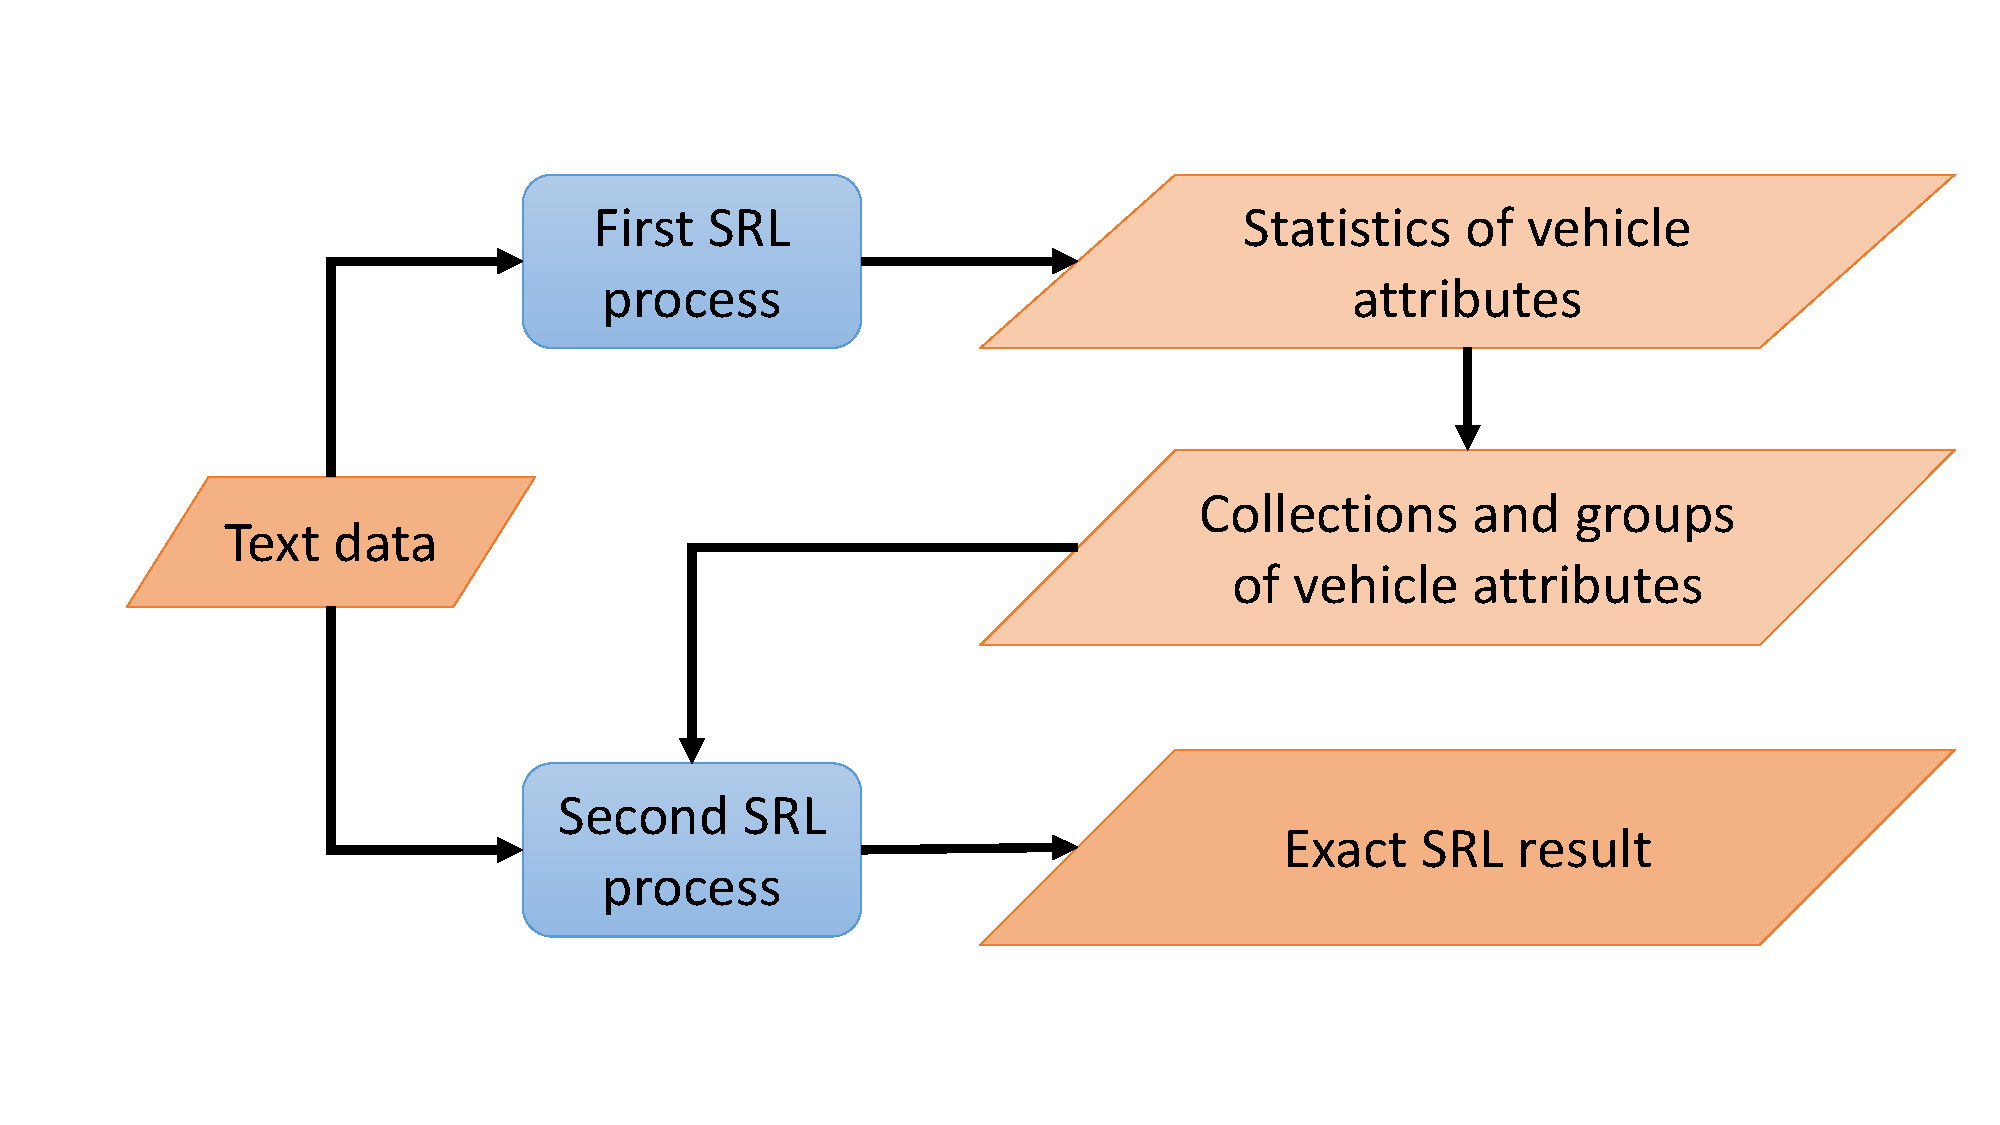
\includegraphics[width=\textwidth]{images/methods/text_branch_overview.pdf}
    \caption{The overview of process flow on text branch.}
    \label{fig:text_branch_overview}
\end{figure}
On such retrieval problems, the text data usually contains rich information about the objects and their activities. Also, this dataset mainly focuses on traffic and vehicle, narrowing the scope of vocabularies but still providing essential information. Therefore, besides feeding the text query into the next-step model, we employ a method to obtain specific query keywords to construct a special collection of vehicle attributes. This task helps us label each query on some categories, useful for later tasks about classification, detector, or re-ranking.
It should be noticed that most of the queries are structured as follow:

\textbf{Vehicle + Action + Optional object(s) + Other information.}

That is the reason we consider English PropBank Semantic Role Labeling (SRL), via the method proposed in \cite{shi2019simple}, as a possibly efficient means to parse verb and noun phrases. A two-phase flow describing the text-branch process is shown in Figure \ref{fig:text_branch_overview}.
\begin{itemize}
    \item First, to analyze the data, we take an SRL extraction on raw data to make statistics on the vehicle's attributes. This process helps us confirm that it is necessary to define potential values about the vehicle types, actions, colors. After filtering the top most frequent and suitable words on each attribute and observing the relation among queries in a track, we create certain groups for three types of the attribute. Figure \ref{fig:group_example} illustrates the result of categorizing.
    \item The second phase of this flow described the heuristic method we build to extract each query on mentioned categories exactly. There are two main stages in this phase, shown in Figure \ref{fig:text_branch_stage_2_overview}.
\end{itemize}

\subsection{Preprocessing stage}
\begin{figure} [!htb]
    \centering
    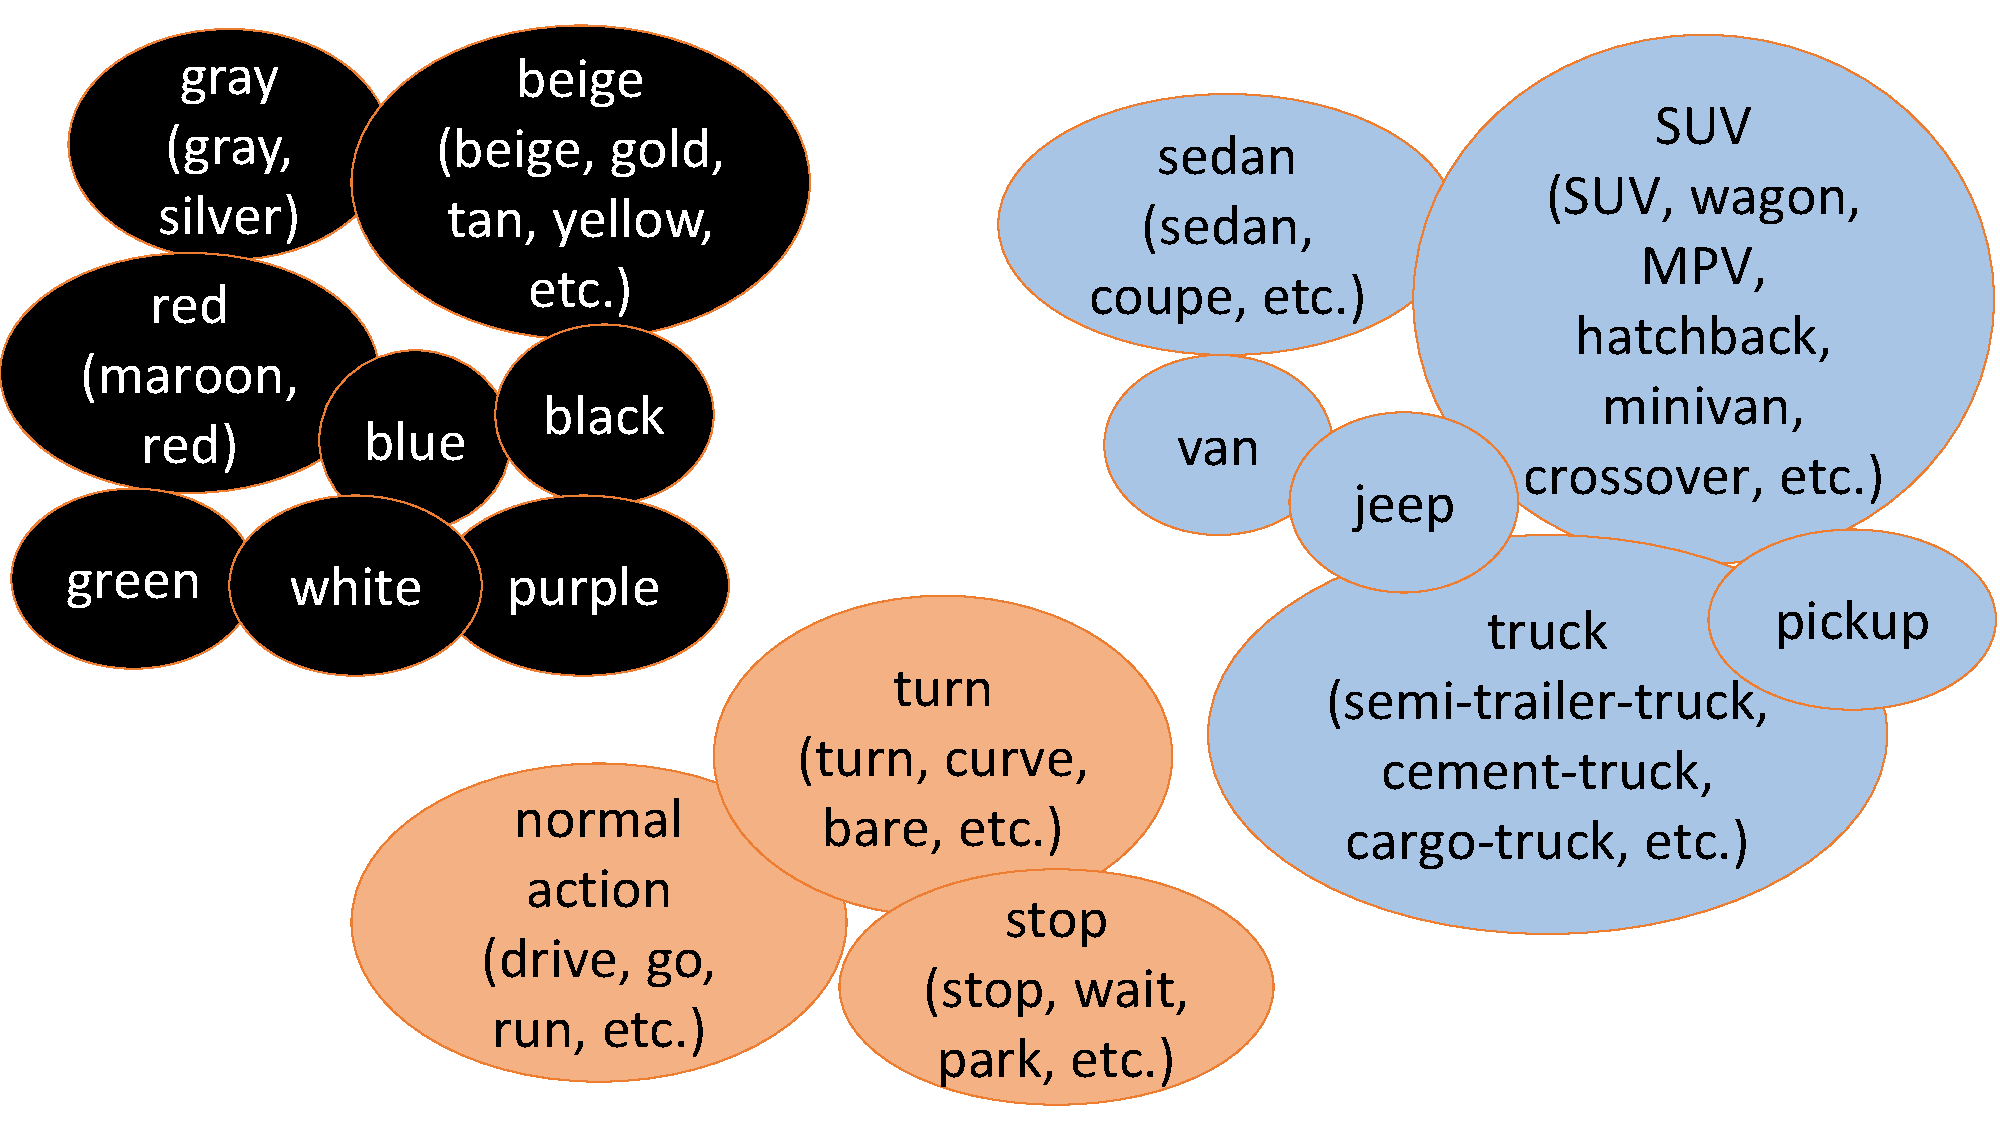
\includegraphics[width=\textwidth]{images/methods/group_example.pdf}
    \caption{How we categorize three attribute types. The black, orange, and blue shapes show the group of color, action, and vehicle type, respectively.}
    \label{fig:group_example}
\end{figure}

\begin{figure}[t!]
    \centering
    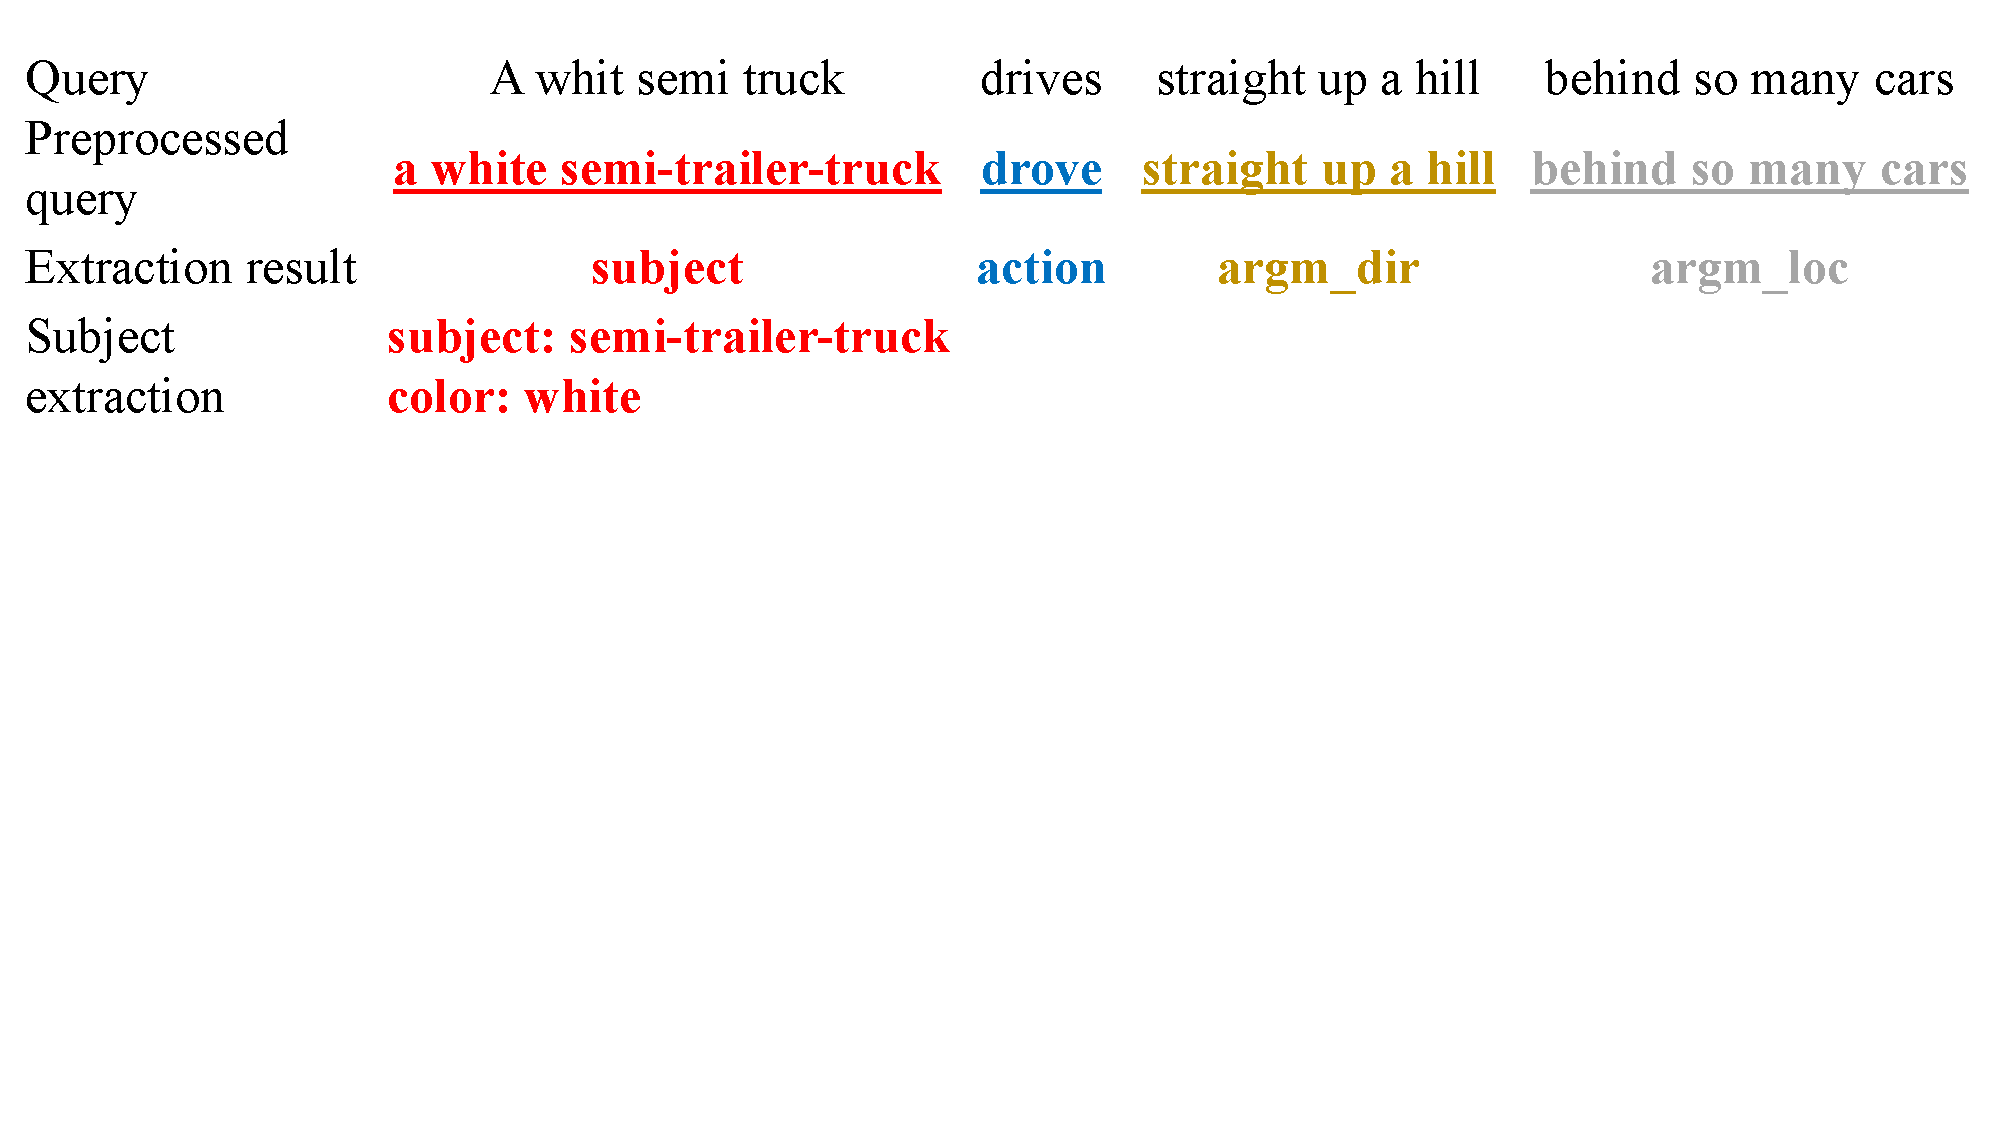
\includegraphics[width=\textwidth]{images/methods/text_extraction_example.pdf}
    \caption{An example of a query transformed and extracted through 2 stages of the heuristics method.}
    \label{fig:text_extraction_example}
\end{figure}
To make the SRL predictor work efficiently, the query needs to be corrected if it has wrong spelling. We use the Levenshtein distance metric to convert a target word to a source word in our defined vocabulary collection of vehicle attributes. To avoid the false convert, we set the condition of correcting a distance equal to 1 between the target word and the source word. We also add a rule to skip certain words which are not misspelled but have a distance of 1. For example, in the preprocessed query provided in Figure \ref{fig:text_extraction_example}, we have changed the wrong word \textit{“whit”} to \textit{“white”} but kept the word \textit{“so”} although it has the Levenshtein distance equal to 1 with the word \textit{“go”}. After this step, there is another collection containing rules to convert inconsistent words or phrases into a common one and/or verbs that are easily confused with nouns into past tense. As seen in the mentioned example, we have also made the word \textit{“semi truck”} (in the same group with \textit{“semi-truck”}, \textit{“tractor-trailer”}) become \textit{“semi-trailer-truck”}, and the word \textit{“drives”} become \textit{“drove”}. When finishing this stage, all of the essential terms related to traffic have been clear enough to be extracted.
\subsection{Extraction stage}
\begin{figure}[!htb]
    \centering
    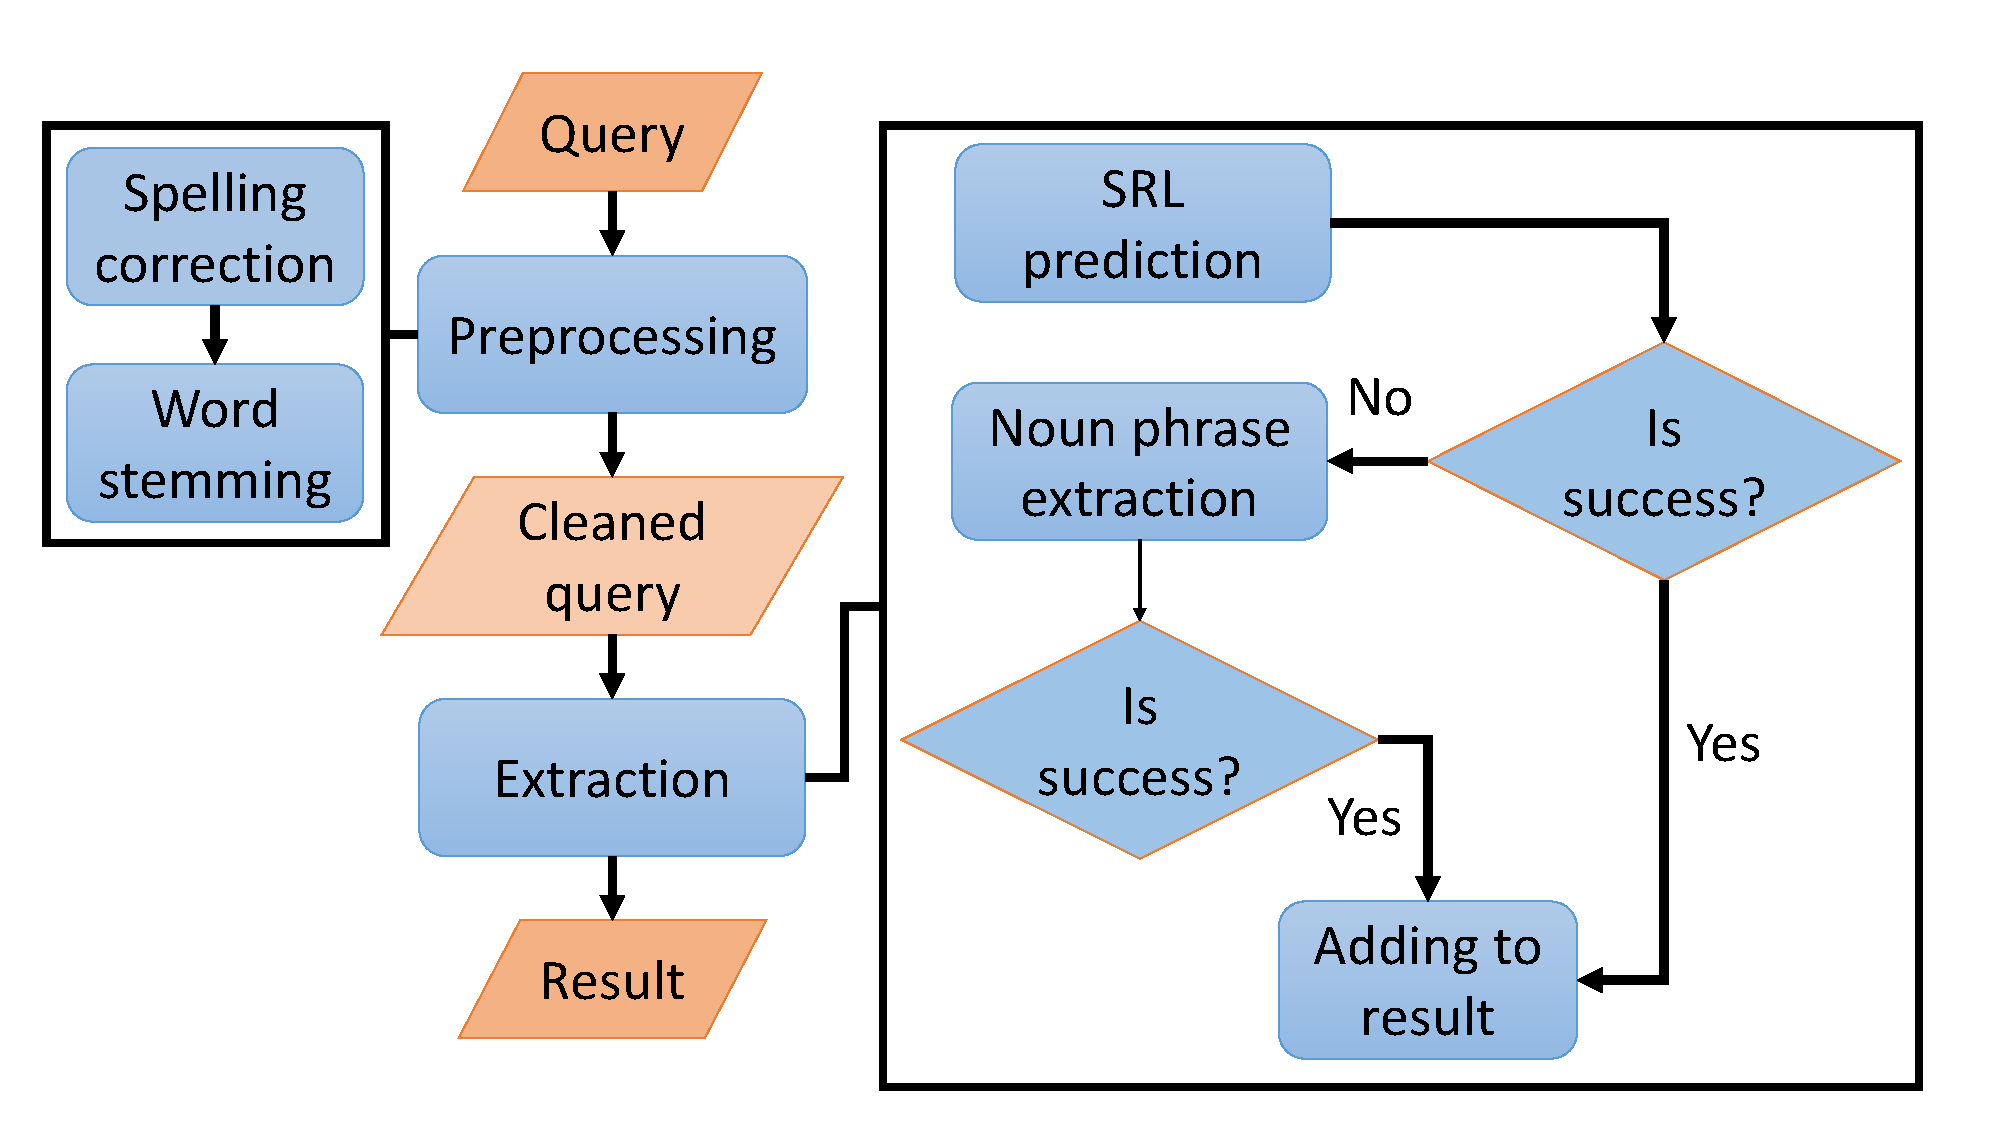
\includegraphics[width=\textwidth]{images/methods/stage_2_overview.pdf}
    \caption{An overview of the heuristic method to extract a query into SRL parts.}
    \label{fig:text_branch_stage_2_overview}
\end{figure}
For each query, a predictor toolkit is used to obtain parts of the SRL result. If the query is a complete sentence, the function will extract successfully. Otherwise, the query can be a noun phrase, and hence we must use another method to handle this. In this situation, we will collect the result if we can find the subject and confirm it as a vehicle type (i.e., \textit{a white truck}, \textit{a typical jeep}), or it will be skipped (i.e., \textit{straight on the main road}, \textit{light short to the right}).


